\documentclass[12pt, a4paper, twoside]{article}

%% Preamble
\usepackage{pdfpages}           % Para incluir PDFs
\usepackage{graphicx}           % Para gráficos
\usepackage{subfiles}           % Para manejar subarchivos
\usepackage{hyperref}           % Para enlaces
\usepackage{listings}           % Para código fuente (ajusta lenguaje)
\usepackage{verbatim}
\usepackage{float}
\usepackage[backend=bibtex,style=numeric]{biblatex} % Para citas numéricas
\addbibresource{references.bib} % Cargar archivo .bib
\usepackage{url}


\usepackage{geometry}           % Para ajustar márgenes

% Ajustes de márgenes
\geometry{
	left=3cm,       % Margen izquierdo
	right=3cm,      % Margen derecho
	top=2.5cm,      % Margen superior
	bottom=2.5cm,   % Margen inferior
	headheight=15pt, % Altura del encabezado
	twoside          % Para documentos a dos caras
}


\graphicspath{{images/}{../images/}} % Ruta para imágenes

\begin{document}
	
	%% Cover
	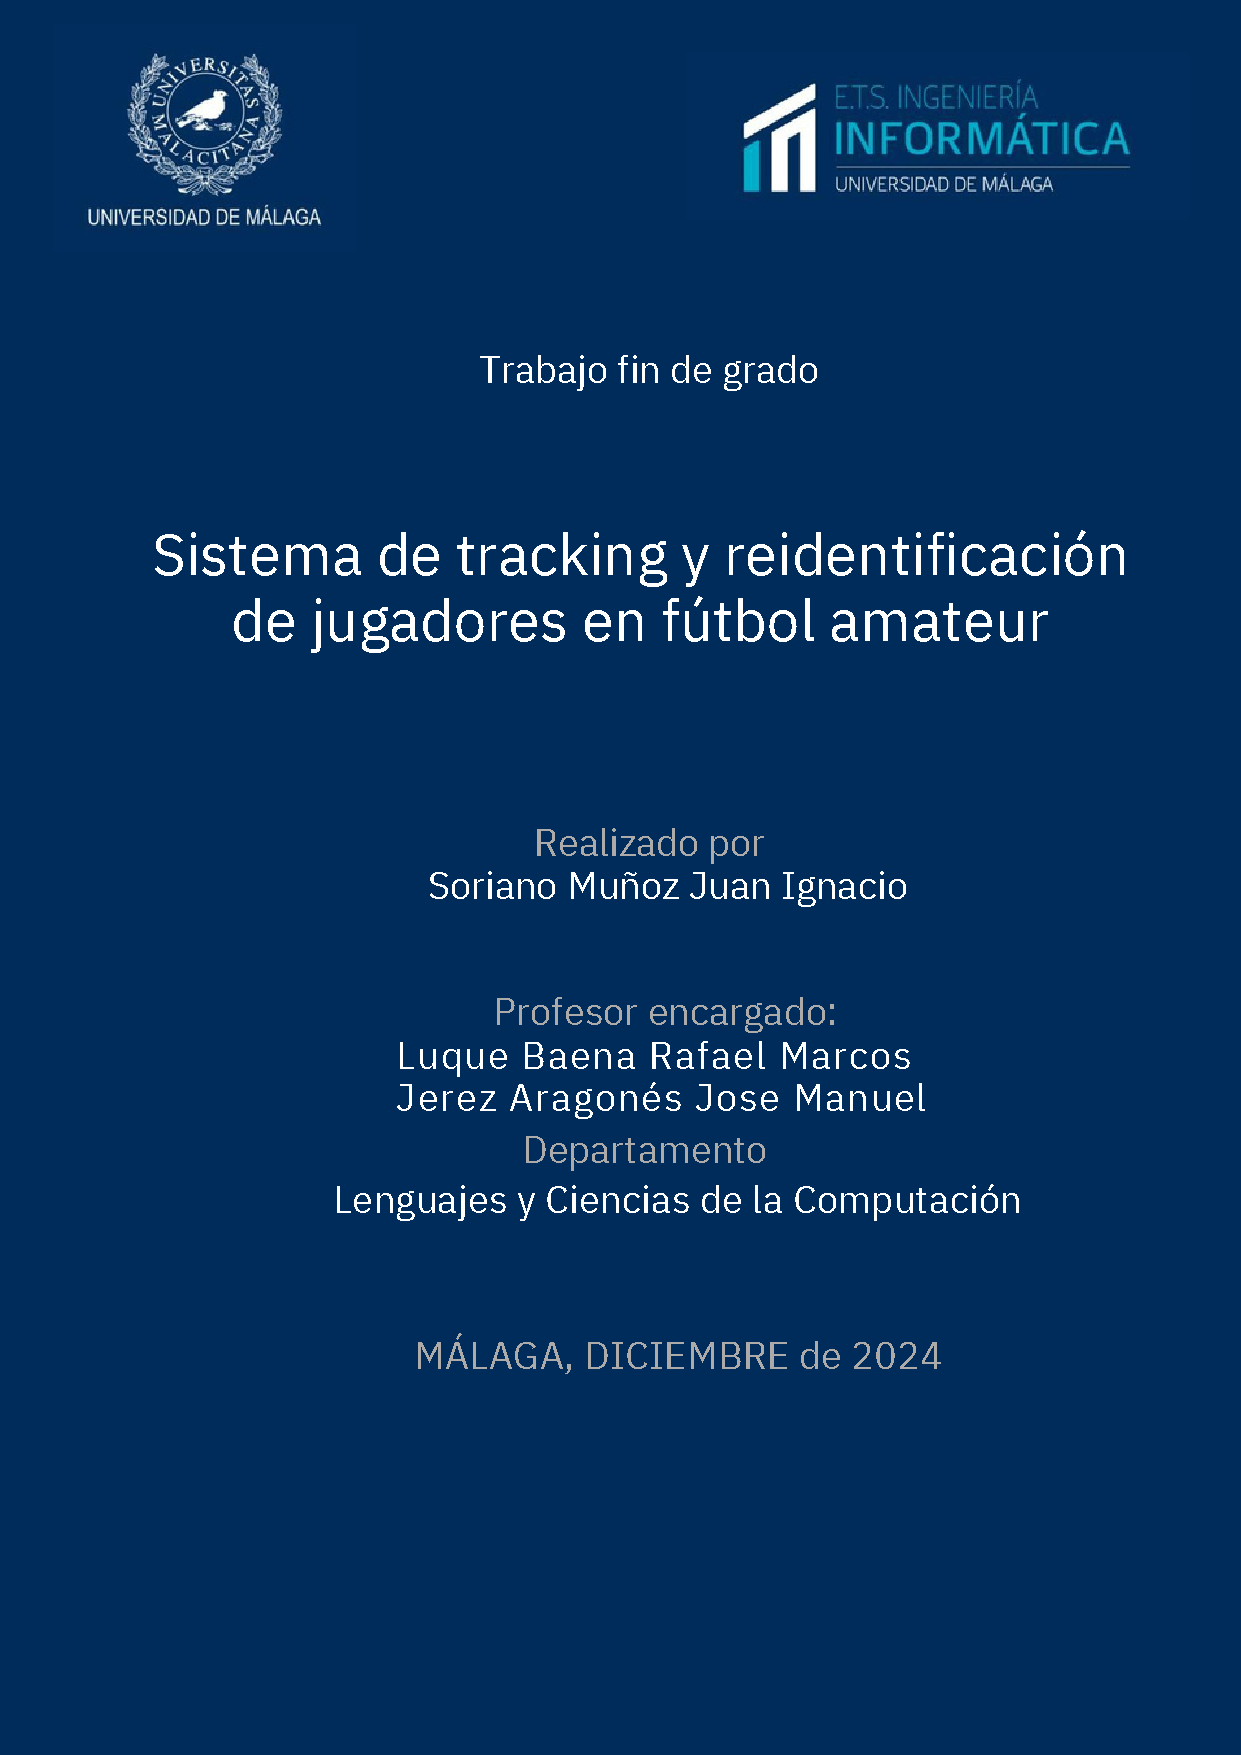
\includepdf[noautoscale=true, width=\paperwidth]{cover.pdf}
	
	%% Title
	\clearpage
	\setcounter{page}{1}
	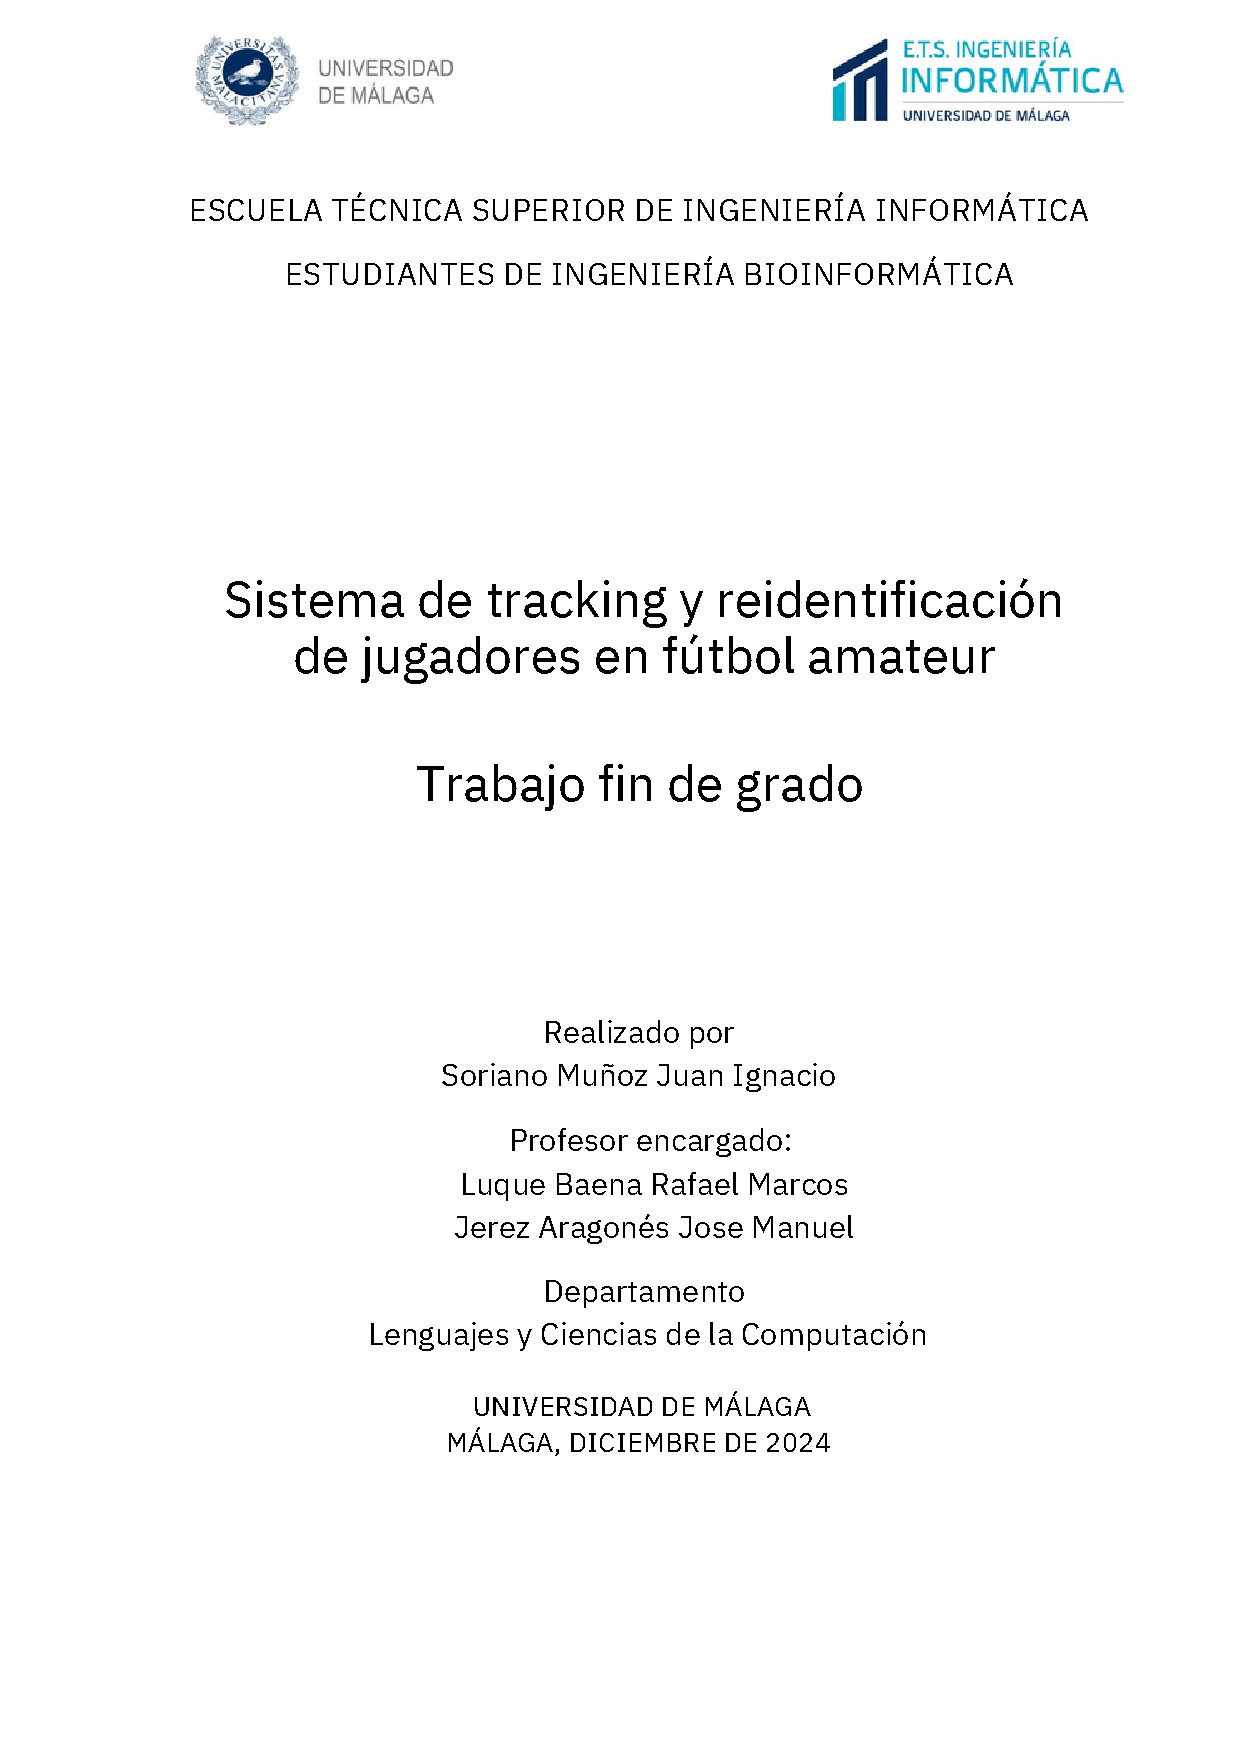
\includepdf[noautoscale=true, width=\paperwidth]{title.pdf}
	
	%%%%%%%%%%%%%%%%%%%%%%%%%%%%%%%%%%%%%%%%%%%%%%%%%%%%%%%%%%%%%%%%%%%%%%%%%%%
	
	% Índice automático
	\tableofcontents
	\newpage
	
	% Sections
	
		% Sections
	\section{Introducción}
	
	\section{Diario de avances}
	
	\subsection{Semana 3-16 de marzo)}
	
	Por ahora lo que llevamos es un dataset hecho en roboflow con un partido de España contra Suiza. Realizamos capturas y dividimos el conjunto en training, validation y test.
	
	Entrené el modelo de YOLO con este dataset revisado y el modelo no supo detectar bien el balón debido a la poca cantidad de imágenes donde se pueda ver bien la bola. El árbitro y los jugadores fueron bien detectados.
	
	Se replanteó el objetivo del TFG. Se focalizará en la reidentificación de jugadores cuando salen fuera de plano y en el desarrollo de una aplicación que permita al usuario decidir si cuando se produce un cambio de identificador, mantenerlo o cambiarlo, creando un dataset revisado.
	
	\subsection{Semana 17-31 de marzo \cite{sun2024gta}}
	
	A la hora de medir resultados como estas gráficas:
	
	\begin{figure}[h]
		\centering
		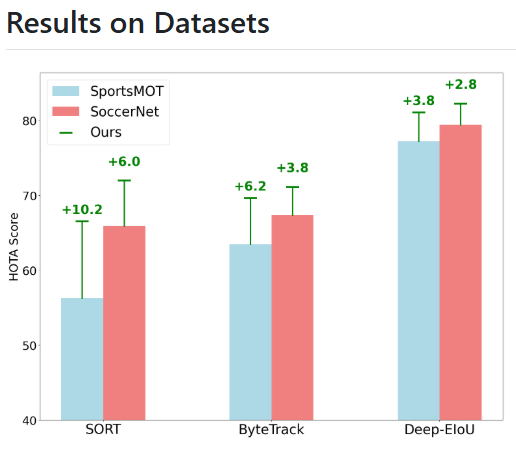
\includegraphics[width=0.8\textwidth]{image/metricasBeta}
		\caption{\textbf{Métricas gta\_link}}
		\label{fig:metricasBeta}
	\end{figure}
	
	Nos centraremos en la medida de los ID's intentando minimizarlos, lo máximo posible, ya que la métrica significa número de ids generados.
	
	\begin{figure}[h]
		\centering
		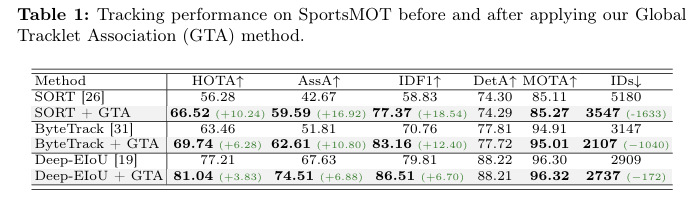
\includegraphics[width=0.8\textwidth]{image/Centrarse}
		\caption{\textbf{Objetivo}}
		\label{fig:Centrarse}
	\end{figure}
	
	Me he puesto a mirar lo que hace exactamente el código del repositorio de gta-link. Y en resumidas cuentas necesitamos un dataset con una pred, ya realizada, como es el caso de SoccerNet. Podemos descargar el dataset con el tracking realizado en los archivos .txt que se encuentran dentro de cada clip.\vspace{0.5cm}
	
	He utilizado las siguientes líneas de comando para realizar la descarga del dataset.
	
	\begin{verbatim}
		from SoccerNet.Downloader import SoccerNetDownloader
		mySoccerNetDownloader = SoccerNetDownloader(LocalDirectory="path/to/SoccerNet")
		mySoccerNetDownloader.downloadDataTask(task="tracking",
		 split=["train","test","challenge"])
	\end{verbatim}
	
	Posteriormente hice unos ajustes en el código para que cogiera los archivos \texttt{gt.txt} para que se tomara como referencia \textbf{--pred\_dir {tracking results directory}}, ya que estos son archivos \textbf{MOT}, que guardan información sobre los \textbf{bounding box} de cada objeto de cada frame, conteniendo información sobre \textbf{frame}, \textbf{id}, \textbf{bb\_left}, \textbf{bb\_top}, \textbf{bb\_width}, \textbf{bb\_height}, \textbf{conf}, \textbf{x}, \textbf{y}, \textbf{z}, en este orden.
	
	Estos son esenciales para que se pueda ejecutar el archivo \texttt{generate\_tracklets.py} para generar los \textbf{tracklets}.
	
	Un \textbf{tracklet} se genera al seguir a un objeto desde su detección en un fotograma hasta el siguiente. En este proceso, el código asocia las detecciones de objetos de cada fotograma con un identificador único (\textbf{ID}) para cada objeto, y los agrupa en una \textbf{"trayectoria"} que sigue ese objeto a lo largo del tiempo.
	
	En el código:
	
	\begin{itemize}
		\item \textbf{Extracción de características:} El código utiliza un modelo de reidentificación de personas (\texttt{FeatureExtractor}) para extraer características visuales de cada objeto detectado en los fotogramas. Esto es útil para seguir objetos entre fotogramas, incluso cuando se producen cambios de apariencia debido a variaciones en la vista o el movimiento.
		\item \textbf{Cálculo de tracklets:} Para cada fotograma, el código agrupa las detecciones de objetos utilizando el identificador único (\texttt{track\_id}). Si un objeto se detecta en un fotograma y luego aparece en otro, se agrega a un tracklet, que es una colección de todas las detecciones del mismo objeto a lo largo de varios fotogramas. Además, se guarda información como el puntaje de la detección y las características extraídas del modelo de reidentificación.
		\item \textbf{Salvado de tracklets:} Al final de cada secuencia de video o serie de fotogramas, los tracklets generados se guardan en un archivo \texttt{pickle} para su posterior uso, permitiendo analizar y trabajar con las trayectorias de los objetos en el futuro.
	\end{itemize}
	
	El programa \texttt{generate\_tracklets.py}, lo que hará será generar unos ficheros \texttt{.pkl} que guardan los datos de las trayectorias de los objetos detectados a lo largo del tiempo. Esto incluye, por ejemplo, las \textbf{detecciones de objetos en cada fotograma}, las \textbf{características extraídas por el modelo de reidentificación}, y los \textbf{identificadores únicos (ID)} asignados a cada objeto (en formato binario).
	
	Una vez que se tenga esos ficheros se realiza una \textbf{refinación de los tracklets} para evitar que se cambien los \textbf{ids con frecuencia}. Mejora los \textbf{tracklets} (trayectorias de objetos) generados por un \textbf{tracker en tareas de seguimiento de múltiples objetos (MOT)}. Utiliza dos componentes principales: el \textbf{Tracklet Splitter}, que divide \textbf{tracklets impuros} (con múltiples identidades) en subtracklets más precisos mediante \textbf{clustering (DBSCAN)}, y el \textbf{Tracklet Connector}, que fusiona \textbf{tracklets fragmentados} que pertenecen al mismo objeto basándose en \textbf{similitudes visuales y restricciones espaciales}. Los resultados refinados se guardan en archivos \texttt{.txt} en formato \textbf{MOT}, listos para su evaluación, visualización o análisis posterior. Este proceso optimiza la \textbf{precisión del seguimiento}, corrigiendo errores como \textbf{cambios de identidad} y \textbf{fragmentaciones}.\vspace{0.5cm}
	
	
	Ahora que tenemos un dataset etiquetado, tendremos que:
	
	\begin{itemize}
		\item \textbf{Encontrar una combinación de hiperparámetros óptima: } Con el objetivo de que el cambio de ids sea el mínimo posible.
		\item \textbf{Desarrollar una aplicación: } Con el objetivo de que avise al usuario sobre los cambios de id en los frames y confirme si está bien cambiado o debería conservarse el anterior.
	\end{itemize}
	
	\subsection{Semana 31-6 de abril)}
	
	En estas semanas hemos estado invirtiendo tiempo en las siguientes cosas. En un principio lo que teníamos era un dataset preparado con los ficheros ground truth fruto de un tracker usado (como DeepEIoU). Pero dado un vídeo, no podíamos aplicar los programas de gta-link, por lo que teníamos que conseguir los ficheros MOT de alguna manera. 
	
	Había dos opciones. La primera aplicar un tracker y la segunda aplicar un modelo de YOLO.
	
	Para la primera opción busqué en varios repositorios, que trataran con trackers, principalmente DeepEIoU, que es el tracker con el mejor rendimiento según las estadísticas de paperscode \cite{sportsmot_paperswithcode}.
	
	\begin{figure}[h]
		\centering
		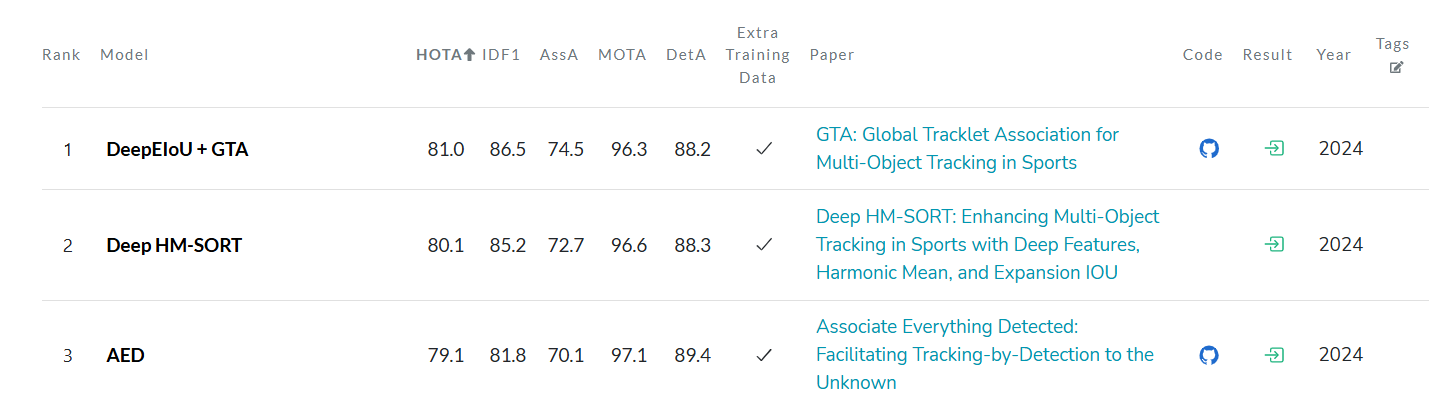
\includegraphics[width=0.8\textwidth]{image/deepEIoU}
		\caption{\textbf{Métricas DeepEIoU}}
		\label{fig:deepEIoU}
	\end{figure} 
	
	Tras encontrar un repositorio que trataba en específico con este \cite{huang2024iterative}. Tuve que modificar código para que utilizara cpu, ya que estaba configurado para gpu de nvidia. Los paquetes no se me instalaban correctamente. Los inputs que utilizaba para los programas eran ficheros tipo .npy.
	
	Dado que me estaba dando muchos problemas, después de dos días decidí que la mejor solución era utilizar un modelo de YOLO. Empecé utilizando un modelo de YOLO estandar capaz de detectar personas. El inconveniente de esto es que el video, estaba grabado desde un ángulo muy bajo, por lo que el modelo detectara las personas de las gradas y esto, a la larga, es un problema. 
	
	Entonces para resolver esto había dos opciones. La primera era realizar una segmentación del campo y la segunda entrenar un modelo de YOLO específico para jugadores. La segmentación del campo es demasiado costosa, porque no hay nada automatizado y sería segmentar infinidad de frames. Además de que es específica para un partido de fútbol en un ángulo en específico.Por lo tanto, la mejor opción para mi gusto es entrenar un modelo de YOLO con un dataset, por ahora, específico del partido de balonmano que me proporcionó mi tutor Jose Manuel Jerez. El dataset lo hice creando un programa utilizando las librerias de opencv (cv2) que extraía frames cada 20 segundos que transcurría de vídeo. Los 20 segundos previenen levemente más overfitting del que ocurre por tener frames del mismo partido. 
	
	Esta opción me permite etiquetar poco, ya que Roboflow tiene una herramienta de etiquetado automático una vez se han etiquetado unas cuantas imágenes, por lo que simplemente tuve que corregir aquellas imágenes con un mal etiquetado.
	
	Tras tener el dataset etiquetado le añadí algunas augmentations. 
	
	A la hora de entrenar el modelo lo hice con 25 epochs. Tardó hora y media en entrenarse.
	
	Apliqué los programas del repositorio de gta-link y los resultados del trackeo son muy buenos, pero la ReID no tiene nada que ver con los resultados tan consistentes del dataset de SoccerNet debido a que la grabación no es profesional.
	
	Aun así tras 23 intentos observe que los parámetros que daban mejores resultados eran los siguientes: --use\_split --min\_len 100 --eps 0.8 --min\_samples 10 --max\_k 4 --use\_connect --spatial\_factor 1.0 --merge\_dist\_thres 0.7   
	
	Recientemente le he añadido frames del partido de fútbol 7 al dataset de roboflow. Y he creado un nuevo modelo de YOLO entrenado exclusivamente con ese dataset.
	
	Los objetivos para la próxima semana:
	
	\begin{itemize}
		\item \textbf{Buscar como aplicar un tracker:} Después de aplicar un trackeo con YOLO, sería necesario aplicar DeepEIoU. Investigar si aplicar un doble gta-link puede funcionar para refinar los tracklets todavía más.
		\item \textbf{Seguir desarrollando la aplicación: } Con el objetivo de que avise al usuario sobre los cambios de id en los frames y confirme si está bien cambiado o debería conservarse el anterior. Ya tengo un programa prueba\_revision\_ReID.py, que funciona como prototipo, pero falta desarrollarlo mucho.
	\end{itemize}
	
	\subsection{Semana 7-13 de abril)}
	
	Al final el proceso de usar el tracker es obligatorio, ya que los objetos son detectados por YOLO, pero luego los ids son colocados por el tracker, y de ahí saldrán ficheros tipo MOT. Entonces tras aplicar YOLO para tener ficheros con la info de los bounding box sobre los jugadores intentaremos aplicarle un tracker y de ahí  un modelo de ReID, para posteriormente utilizar gta.
	
	Secuencia de trabajo: YOLO + DeepEIoU + GTA
	
	\subsection{Semana 7-13 de abril)}
	
	Planteé una estructura oficial de lo que llevo hecho para que sea más formal y dar contexto e información sobre todo lo que rodea las prácticas y el proyecto de TFG.
	
	\section{Motivación y Contexto}
	
	\subsection{¿Por qué es importante el análisis en fútbol amateur?}
	
	El análisis de rendimiento, la estadística avanzada y el seguimiento de jugadores han revolucionado el fútbol profesional. Sin embargo, en el fútbol amateur estas tecnologías todavía son muy poco accesibles.
	Poder aplicar técnicas de tracking y análisis en estos niveles permitiría:
	\begin{itemize}
		\item \textbf{Mejorar el entrenamiento de jugadores jóvenes.}
		\item \textbf{Facilitar la toma de decisiones a entrenadores y clubes pequeños.}
		\item \textbf{Promover el desarrollo del talento de forma más justa y basada en datos.}
	\end{itemize}
	
	\subsection{¿Qué problema hay actualmente?}
	
	La causa del primer problema que encontramos es la deficiencia en las infraestructuras tecnológicas para la práctica del fútbol amateur; el hecho de no disponer de sistemas avanzados que implementan las cámaras múltiples o los sensores del fútbol en el sector profesional, por el alto coste que implicaría el uso de las soluciones comerciales de tracking (GPS, cámaras VICON, sistemas ópticos, etc.) y la escasez de datos de movimiento y rendimiento que sufren las categorías base y amateur.
	
	\section{Objetivos}
	
	El presente proyecto tiene como principal objetivo colaborar en el análisis de los deportes a nivel de fútbol amateur implementando un sistema de detección automática, de seguimiento y de reidentificación de los jugadores. A día de hoy, existe una diferencia muy considerable entre la tecnología que existe para el análisis táctico y de rendimiento del fútbol profesional y la del ámbito amateur, lo cual significa que clubes, entrenadores y jugadores amateurs no tienen las herramientas disponible para realizar un análisis automatizado y estructurado de sus partidos.
	Este trabajo pretende eliminar esta desigualdad creando un flujo de trabajo modular y eficiente que permita aplicar tecnología avanzada de visión por computador en el ámbito amateur. Para ello se combinan modelos de detección de objetos (YOLOX) con algoritmos de seguimiento multiobjeto (DeepEIoU) y técnicas de reidentificación de personas (ReID) con el modelo OSNet, las cuales son reforzadas con un refinamiento posterior (GTA-Link) que mejora la calidad de las trayectorias generadas.
	
	Los objetivos específicos del proyecto son los siguientes:
	
	\begin{itemize}
		\item Desarrollar un sistema capaz de identificar y seguir automáticamente a los jugadores durante el transcurso de un partido de fútbol grabado en vídeo.
		\item Implementar un modelo de reidentificación que permita mantener la coherencia de los IDs incluso ante desapariciones temporales del jugador en la escena.
		\item Aplicar técnicas de post-procesamiento para corregir errores comunes en los tracklets generados, como fragmentación o mezcla de identidades.
		\item Facilitar la reutilización y escalabilidad del flujo de trabajo en otros entornos deportivos, fomentando así su adopción por parte de entidades del fútbol base o amateur.
		\item Probar y validar el sistema sobre secuencias reales de fútbol amateur, evaluando su rendimiento en condiciones no controladas.
	\end{itemize}

	
	\section{Estado del sector}
	
	El análisis de rendimiento en el fútbol ha experimentado una transformación significativa en las últimas décadas, impulsada por avances tecnológicos que permiten una recopilación y procesamiento de datos cada vez más precisos y en tiempo real. Sin embargo, existe una marcada diferencia entre las herramientas utilizadas en el ámbito profesional y las accesibles para equipos amateurs.
	
	\subsection{Soluciones en el Ámbito Profesional}
	
	En el fútbol profesional, sistemas como TRACAB se han consolidado como referentes en el seguimiento y análisis de jugadores. TRACAB es un sistema de seguimiento óptico que utiliza cámaras y algoritmos de visión por computadora para rastrear en tiempo real la posición de todos los jugadores y el balón en el campo. Este sistema ha sido implementado en ligas de élite como la Premier League, La Liga y la Bundesliga, y está certificado por la FIFA para programas de seguimiento electrónico de rendimiento (EPTS). "https://tracab.com/products/tracab-technologies/?utm\_source=chatgpt.com"
	
	\subsection{Herramientas Disponibles para el Fútbol Amateur}
	
	En contraste, el fútbol amateur ha comenzado a adoptar herramientas más asequibles y adaptadas a sus necesidades y recursos. Una de las más destacadas es LongoMatch, un software de análisis de vídeo que permite a entrenadores y analistas etiquetar eventos, crear estadísticas y generar informes tácticos a partir de grabaciones de partidos.
	
	LongoMatch ofrece "https://longomatch.com/en/?utm\_source=chatgpt.com":
	\begin{itemize}
		\item	Análisis en tiempo real y post-partido con soporte para múltiples cámaras.

	
		\item Personalización de paneles de análisis según las necesidades del equipo.
	
		\item Exportación de datos y vídeos para compartir con jugadores y cuerpo técnico.
	
		\item Compatibilidad con diversas plataformas y dispositivos móviles.
	\end{itemize}
	
	Además, herramientas como PIX4TEAM 2 han emergido para automatizar la grabación de partidos sin necesidad de un operador de cámara, facilitando la recopilación de material para análisis en equipos con recursos limitados. "https://shop.movensee.com/es/content/31-pix4team-camara-automatica-para-los-deportes-colectivos"
	
	\subsection{Limitaciones}
	
	\begin{center}
		\begin{tabular}{|p{6.5cm}|p{6.5cm}|}
			\hline
			\textbf{Limitaciones del sector amateur} & \textbf{Aportaciones del presente proyecto} \\
			\hline
			Los sistemas comerciales como Second Spectrum o STATS SportVU requieren múltiples cámaras y hardware costoso. &
			Se utiliza vídeo monocámara accesible y fácil de capturar con dispositivos comunes. \\
			\hline
			Los trackers convencionales pierden frecuentemente la identidad del jugador en escenas con oclusiones o cambios de plano. &
			Se implementa un módulo de re-identificación (ReID) basado en TorchReID y OSNet para mantener la identidad a lo largo del partido. \\
			\hline
			No existen herramientas que generen anotaciones automáticas de forma sencilla a partir del vídeo. &
			Se desarrolla un flujo de trabajo que genera archivos de anotaciones (formato MOT) automáticamente a partir del vídeo de entrada. \\
			\hline
			Los modelos existentes están entrenados en entornos profesionales, con condiciones muy diferentes al fútbol amateur. &
			Los modelos utilizados en este proyecto han sido entrenados y validados específicamente sobre partidos de fútbol amateur. \\
			\hline
			Las soluciones actuales no están diseñadas para clubes pequeños: requieren licencias, suscripciones o personal técnico. &
			Se busca una solución reproducible, ligera y gratuita basada en herramientas \textit{open-source}, accesible a cualquier usuario técnico. \\
			\hline
		\end{tabular}
	\end{center}
	
	\section{Tecnologías empleadas}
	
	Este proyecto ha hecho uso de diversas tecnologías de software y frameworks de inteligencia artificial que permiten implementar un sistema de tracking con detección, seguimiento y reidentificación de jugadores en partidos de fútbol amateur. A continuación, se detallan las principales herramientas y recursos utilizados.
	
	\subsection{Programación}
	
	Para el desarrollo del sistema se ha utilizado el lenguaje de programación Python, por su gran ecosistema de librerías para visión por computadora y deep learning. El flujo de trabajo se ha dividido en diferentes etapas, desarrolladas principalmente en entornos Jupyter Notebook y scripts de Python:
	
	\begin{itemize}
		\item \textbf{Jupyter Notebook:} Se utilizó para entrenar el modelo de detección de objetos YOLO, aprovechando la facilidad para experimentar de forma interactiva con parámetros y visualizar resultados.
		\item \textbf{Python (scripts):} Fue empleado para el entrenamiento del modelo de re-identificación (ReID), así como para aplicar todos los modelos en el flujo final de inferencia y generación de vídeos etiquetados con las predicciones.
	\end{itemize}
	
	\subsection{Gestión de datos y flujo de trabajo}
	
	\textbf{Roboflow} ha sido una herramienta fundamental para gestionar el dataset de entrenamiento del detector YOLO. Roboflow permite subir imágenes, etiquetarlas, realizar aumentos de datos automáticamente y exportar el dataset en el formato deseado (en nuestro caso, YOLOv8).
	
	\textbf{GitHub} ha sido el sistema elegido para el control de versiones y colaboración. Se ha utilizado para organizar y almacenar los diferentes módulos del proyecto, así como mantener un historial ordenado de los avances y pruebas realizadas durante el desarrollo del TFG.
	
	\subsection{Modelos utilizados}
	
	\textbf{YOLO (You Only Look Once)} ha sido el modelo principal utilizado para la detección de jugadores. Su arquitectura permite realizar detección en tiempo real, con una alta precisión y bajo coste computacional. Se entrenó una versión ligera del modelo con imágenes de fútbol amateur obtenidas del dataset gestionado en Roboflow.
	
	\textbf{DeepEIoU} fue el algoritmo de tracking utilizado para asociar detecciones entre frames y mantener la identidad de cada jugador. DeepEIoU combina estrategias geométricas (IoU) y de apariencia (cuando se usa ReID), lo que mejora la robustez frente a oclusiones y cambios de plano.
	
	Este modelo ha sido clave para generar archivos de anotación con los ID temporales de los jugadores a lo largo del vídeo, y servir como base para el post-procesamiento posterior mediante GTA-Link.
	
	\textbf{TorchReID} se ha usado como framework para entrenar el modelo de re-identificación. Se utilizó el modelo \textit{osnet\_x1\_0}, que fue ajustado sobre imágenes recortadas de jugadores, organizadas en carpetas según su identidad. Este modelo se utilizó posteriormente para mejorar el seguimiento, reduciendo los cambios de identidad.
	
	
	
	\section{Módulo de detección (YOLO)}
	https://arxiv.org/abs/1506.02640
	
	\subsection{Arquitectura YOLO}
	
	YOLO (You Only Look Once) es una arquitectura de detección de objetos en imágenes y vídeos que ha destacado por su velocidad y precisión. La arquitectura original de YOLO, según la propuesta en el artículo de Redmon et al. (2016)\footnote{Redmon, J., Divvala, S., Girshick, R.,  Farhadi, A. (2016). You Only Look Once: Unified, Real-Time Object Detection. arXiv preprint arXiv:1506.02640.}, se inspira parcialmente en GoogleNet y está compuesta por 24 capas convolucionales, cuatro capas de agrupamiento máximo (max pooling) y dos capas totalmente conectadas al final.
	
	Antes de procesarse, la imagen de entrada es redimensionada a un tamaño fijo de 448x448 píxeles. El flujo interno de la red emplea convoluciones de tipo 1x1 que tienen como función principal reducir el número de canales de activación intermedios sin afectar a la información espacial. Posteriormente, se aplican convoluciones de 3x3 para capturar patrones locales más complejos. Cada una de estas capas es seguida por una función de activación ReLU, que introduce no linealidad al modelo, excepto en la capa de salida, donde se emplea una función de activación lineal.
	
	Además, para mejorar la estabilidad del entrenamiento y evitar el sobreajuste, se aplican técnicas como la normalización por lotes (Batch Normalization) y el abandono (Dropout). Estas estrategias permiten que el modelo generalice mejor ante nuevos datos y se mantenga robusto frente a variaciones del entorno.
	
	Esta arquitectura permite que YOLO realice detección de múltiples objetos en una sola pasada sobre la imagen (de ahí su nombre), lo que lo convierte en un modelo extremadamente eficiente para tareas en tiempo real.
	
	\subsection{¿Cómo funciona la detecci\'on de objetos con YOLO?}
	
	Una vez entendida la arquitectura interna de YOLO, es importante comprender cómo se lleva a cabo el proceso de detección de objetos. Para ello, se puede imaginar el caso práctico de una aplicación que detecta jugadores y balones de fútbol a partir de una imagen de vídeo.
	
	\begin{figure}[H]
		\centering
		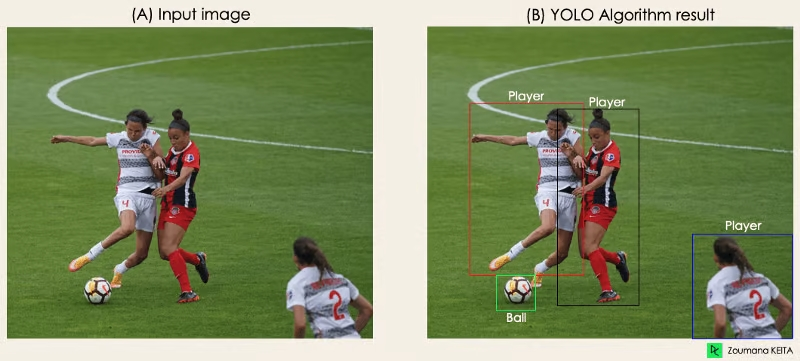
\includegraphics[width=0.8\textwidth]{image/yolodec1}
		\caption{\textbf{YOLO Detection. First Step}}
		\label{fig:YOLO Detection. First Step}
	\end{figure}
	
	El algoritmo de detección en YOLO se basa en cuatro pilares fundamentales: la división en cuadrículas, la regresión de cajas delimitadoras (bounding boxes), el cálculo del coeficiente de intersección sobre unión (IoU), y la supresión no máxima (NMS).
	
	\begin{enumerate}
		\item \textbf{División en cuadrículas (bloques residuales):} La imagen de entrada se divide en una cuadrícula de tamaño $N\times N$, donde cada celda es responsable de detectar los objetos que contiene. Cada celda predice una clase y una probabilidad asociada, además de parámetros que definen la caja delimitadora. 
		
		\begin{figure}[H]
			\centering
			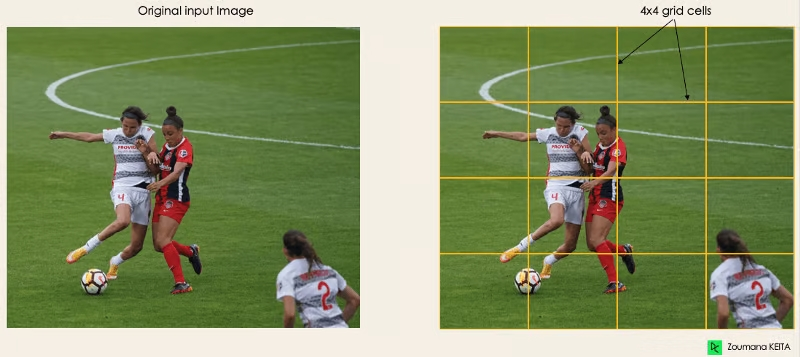
\includegraphics[width=0.8\textwidth]{image/yolodec2}
			\caption{\textbf{YOLO Detection. Second Step}}
			\label{fig:YOLO Detection. Second Step}
		\end{figure}
		
		
		\item \textbf{Regresión de cajas delimitadoras:} Cada celda predice varias cajas en el formato $Y = [p_c, b_x, b_y, b_h, b_w, c_1, c_2, \dots, c_n]$, donde:
		\begin{itemize}
			\item $p_c$ es la probabilidad de que la celda contenga un objeto.
			\begin{figure}[H]
				\centering
				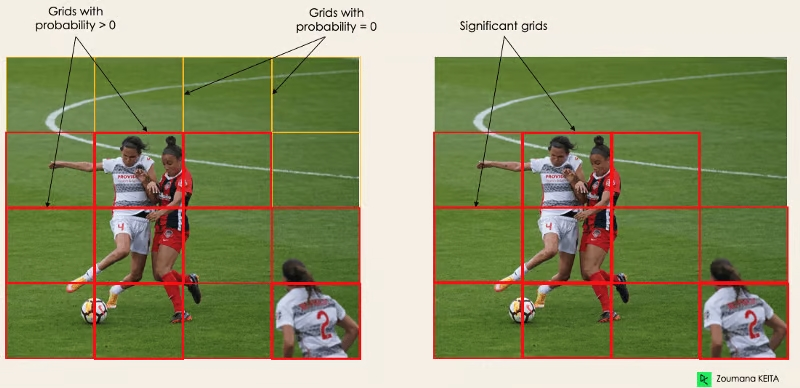
\includegraphics[width=0.8\textwidth]{image/yolodec3}
				\caption{\textbf{YOLO Detection. Third Step}}
				\label{fig:YOLO Detection. Third Step}
			\end{figure}
			\item $b_x$, $b_y$ son las coordenadas del centro de la caja respecto a la celda.
			\item $b_h$, $b_w$ son la altura y la anchura de la caja.
			\item $c_1, c_2, \dots$ son las probabilidades de pertenencia a cada clase (jugador, balón, etc.).
		\end{itemize}
		
		\begin{figure}[H]
			\centering
			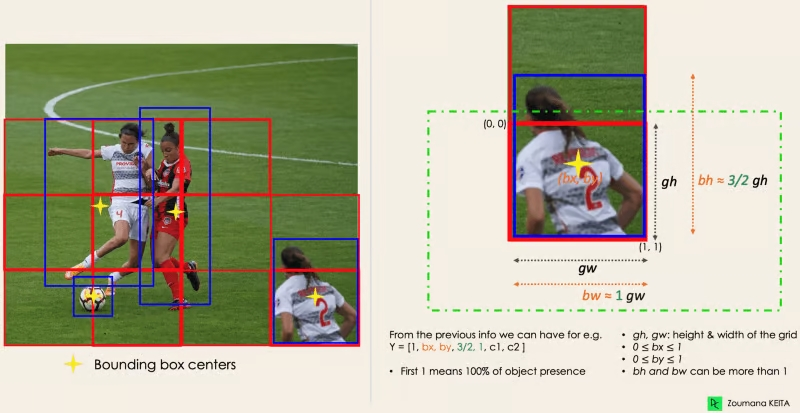
\includegraphics[width=0.8\textwidth]{image/yolodec4}
			\caption{\textbf{YOLO Detection. Fourth Step}}
			\label{fig:YOLO Detection. Fourth Step}
		\end{figure}
		
		
		
		
		\item \textbf{Intersección sobre Unión (IoU):} Para cada predicción, YOLO calcula el solapamiento entre la caja predicha y las cajas reales (ground truth). El valor del IoU (entre 0 y 1) permite descartar predicciones de baja calidad. Sólo aquellas con un IoU superior a un umbral son tenidas en cuenta.
		
		\begin{figure}[H]
			\centering
			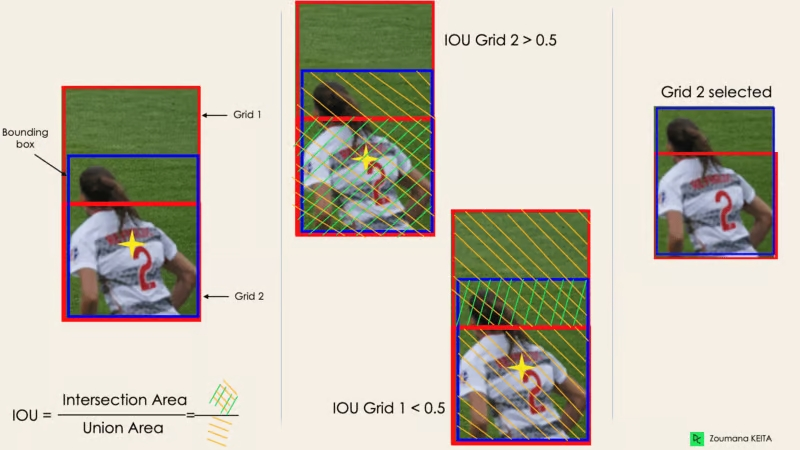
\includegraphics[width=0.8\textwidth]{image/yolodec5}
			\caption{\textbf{YOLO Detection. Fifth Step}}
			\label{fig:YOLO Detection. Fifth Step}
		\end{figure}
		
		
		\item \textbf{Supresión No Máxima (NMS):} Cuando varias cajas se solapan con valores altos de IoU, el algoritmo aplica NMS para conservar sólo la de mayor probabilidad, eliminando duplicados y reduciendo el ruido en las predicciones.
	\end{enumerate}
	
	Este proceso completo permite que, en un único paso y de forma muy eficiente, YOLO identifique múltiples objetos en una imagen, indicando su clase y ubicación precisa. Esta capacidad lo convierte en una herramienta especialmente útil en el análisis de vídeo deportivo, donde se requiere detectar varios jugadores en escenas rápidas y dinámicas.
	"https://www.datacamp.com/blog/yolo-object-detection-explained"
	
	
	\section{Módulo de tracking + Gestión de IDs}
	
	
	\subsection{Módulo de tracking}
	En el contexto de la detección de objetos en vídeo, como la realizada por modelos como YOLO, cada fotograma es procesado de forma independiente. Esto significa que, aunque el detector puede identificar y localizar objetos en cada imagen, no mantiene información sobre la identidad de estos objetos a lo largo del tiempo. Por ejemplo, no puede determinar si el jugador detectado en el fotograma 1 es el mismo que en el fotograma 2.
	
	Para abordar esta limitación, se emplean algoritmos de seguimiento de objetos (trackers) que asocian las detecciones entre fotogramas consecutivos, permitiendo así mantener la identidad de cada objeto a lo largo del tiempo. Estos trackers asignan un identificador único a cada objeto y actualizan su posición en cada nuevo fotograma, incluso en presencia de oclusiones o cambios de apariencia.
	
	Un ejemplo destacado de este enfoque es el algoritmo Deep SORT (Simple Online and Realtime Tracking with a Deep Association Metric), que combina información de movimiento y apariencia para asociar detecciones entre fotogramas. Deep SORT utiliza un filtro de Kalman para predecir la posición futura de los objetos y un descriptor de apariencia basado en redes neuronales profundas para comparar similitudes visuales entre detecciones. La asociación entre detecciones y trayectorias se realiza mediante el algoritmo húngaro, que minimiza el coste total de asociación considerando tanto la distancia de movimiento como la similitud de apariencia.
	"https://doi.org/10.1109/ICIP.2017.8296962"
	
	\subsection{Gestión de IDs}
	
	"https://paperswithcode.com/task/person-re-identification"
	
	La Re-identificación de Personas es una tarea de visión por computadora cuyo objetivo es asociar la identidad de una persona a través de diferentes cámaras o ubicaciones en una secuencia de vídeo o imágenes. Implica detectar y seguir a una persona y luego utilizar características como apariencia, forma del cuerpo y ropa para asociar su identidad en diferentes fotogramas. El objetivo es asociar a la misma persona en múltiples vistas de cámara no superpuestas de manera robusta y eficiente. 
	
	
	\section{Propuesta}
	
	\begin{figure}[H]
		\centering
		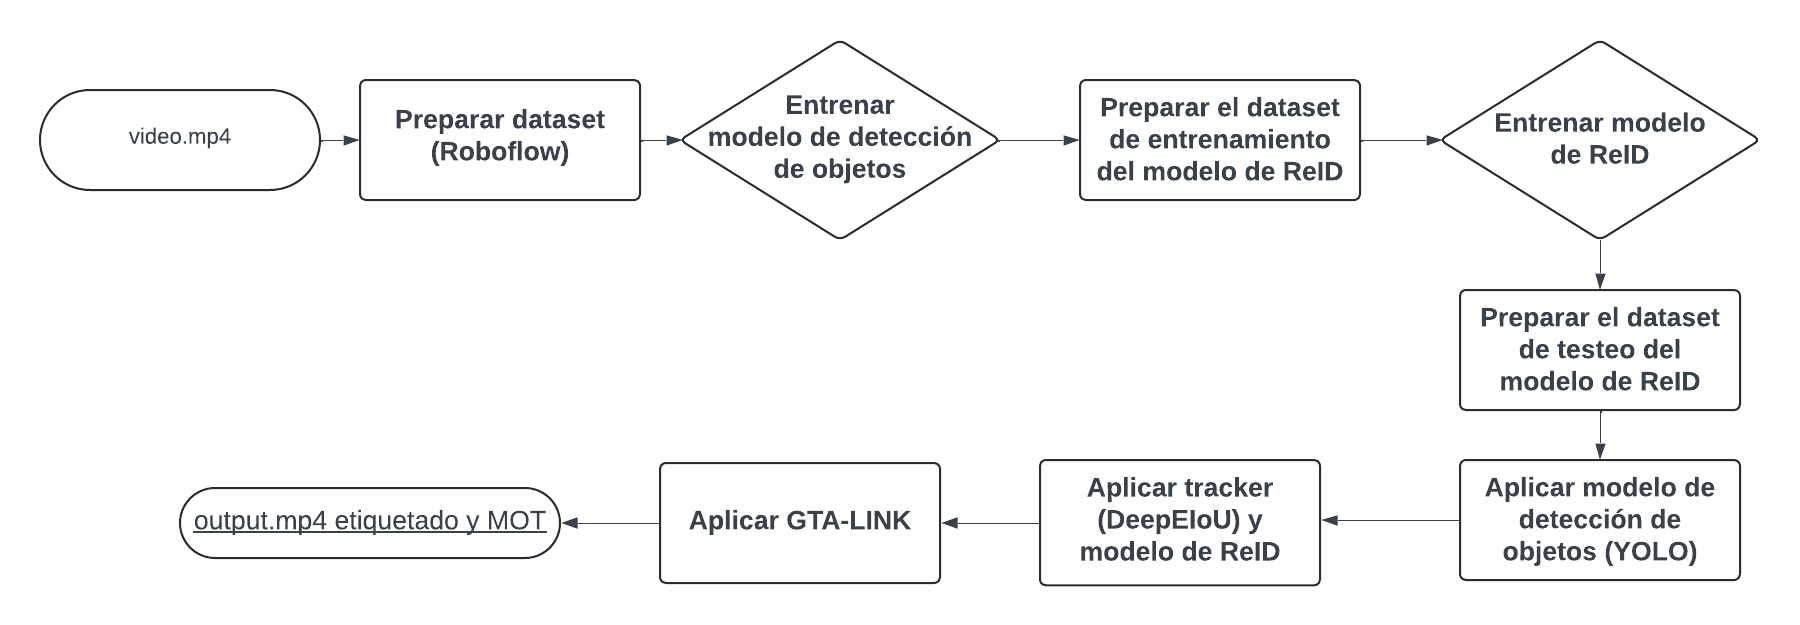
\includegraphics[width=0.8\textwidth]{image/Flowcharts}
		\caption{\textbf{Propuesta}}
		\label{fig:Propuesta}
	\end{figure}
	
	\section{Arquitectura general del sistema}
	
	
	\section{Resultados Preliminares}
	
	
	\section{Dificultades encontradas}
	
	
	\section{Conclusiones}
	
	
	
	%%%%%%%%%%%%%%%%%%%%%%%%%%%%%%%%%%%%%%%%%%%%%%%%%%%%%%%%%%%%%%%%%%%%%%%%%%%
	\printbibliography
	
	
	%% Back Cover
	
\includepdf[noautoscale=true, width=\paperwidth]{backcover.pdf}
	
\end{document}